\documentclass[12pt,journal,compsoc]{IEEEtran}

\usepackage[margin=1in]{geometry}

\title{CovertFS Implementation}
\author{Ryne~Flores, Kyle~Gorak, David~Hart, Matthew~Sjoholm, LTC Timothy Nix \\ \IEEEmembership{Department of Electrical Engineering and Computer Science\\ United States Military Academy}}
\IEEEtitleabstractindextext{
\begin{abstract}
In 2007 Arati Baliga, Joe Kilian, and Liviu Iftode of Rutgers University presented the idea of a web based covert file system~\cite{Baliga2007}. The purpose of a web based covert file system is providing confidentiality and plausible deniability regarding the existence of files. The key components of a web based covert file system is hiding files within media using steganographic techniques using online file sharing for the purpose of collaboration~\cite{Baliga2007}. We created such a system, covertFS, as a prototype to develop the idea for a web based covert file system previously mentioned. Our prototype of the web based covert file system implements steganographic techniques to obfuscate an entire file system on a public file share site. By storing data in this manner, rather than within the application or on a users computer, we provide confidentiality and plausible deniability to both the users and the companies that manage these public file sharing sites. 
\end{abstract}}
\date{}

\begin{document}
\maketitle

\section{Introduction}

%\IEEEPARstart{T}{he} main purpose of a web-based covert filesystem is to attempt to develop an environment that allows uses to store and share information with one another in a more discreet and private manner. Technology continues to advance at a rapid pace, and its advancements are making their way into nearly everything we use and wear. 

\IEEEPARstart{T}{echnology} continues to integrate itself more and more in our daily lives because of the convenience it provides to users. Users are becoming connected to the internet in multiple ways nearly everywhere they go. Numerous devices are being developed and released to provide more convenience to users and to keep them updated on their various interests. A user will usually have at the very least a cell phone on their person and throughout their routine on any particular day will browse email, social media sites, and various other applications. These applications themselves, regardless of the convenience they provide users, can track and offer the user the option to post their information on the user's social media site profile to share among friends and acquaintances 

The majority of people interact with various forms of technology throughout each day. Depending on what type of technology we interact with there may be some type of data collected from our interaction. Also the use of social media is wide spread and it is easier to find various types of information about people because of this. 

The means to store and share information in a covert manner not only serves multiple purposes, but also has various implications depending on how those means are used. There will be innovations designed with the good intentions, yet there will also usually be clever modifications of those designs for malicious intentions.

This project is an application that allows users to share information in a covert manner that can provide plausible denaibility to not only the users but also to the file sharing or social media site that is being used as a medium where the information is stored.

\section{Related Works}
There are other projects and systems that have been released which offer users covert methods of sharing information. Such examples include Tor and StegFS\cite{Tan2003}. The main concepts of this project were obtained from a paper that which invovled faculty and students from Rutgers University\cite{Baliga2007}.  There has been no other implementation of the application described in the Rutger's paper, and this project is our take at creating a working prototype which could later be used to develop a successful application or implementation of the covert file system.

%Yet by entering the covert realm of the internet we are allowing our project to criticized on the ethics of it development in accordance with ACM code of Ethics and Professional Conduct\cite{Anderson1993}. Just as Tor is reviewed arguments are brought up against further development\cite{Guitton2013} so to may this project draw vast attention because of what it offers or means to malicious users and intentions.

\section{Design Overview}

In this section we will explain how we decided to implement a prototype of this project.

\subsection{Web Connection}

Our application's interface with the internet needs to serve three purposes:
\begin{enumerate}
\item Retrieve pseudo random images to use for embedding a message. 
\item Upload images to a public online forum anonymously without altering the image.
\item Retrieve specific images from a public online forum anonymously without altering the image. 
\end{enumerate}

After some research, we discovered a service that could satisfy the first purpose. The Cat API provides random cat images retrieved from Tumblr. The API is reliable and returns content neutral images big enough to store information. A downside to this approach is that statistical steganalysis can be done to compare the uploaded images to the originals. The possibility of using local unique images is out of the scope of our project. The next two requirements are fulfilled by Sendspace.com. This website provides an external API that allows our application to easily interface with and upload and download full size images anonymously. 

%The only significant issue that we encountered while using these online resources was with Sendspace.
% At some point, Sendspace updated their API to require a key. We were not aware of this update and our application was completely broken until we found the bug and fixed it.

The online resources work together as follows:
\begin{enumerate}
\item The Cat API retrieves a random cat image for a message to be embedded into.
\item Embed data into image.
\item Upload the encoded image to Sendspace. Sendspace returns and download and delete URL.
\item Download the encoded image using the download URL.
\item Decode the image to restore original data. 
%This allows for the retrieval of the original message. 
\end{enumerate}

\subsection{FUSE}

What FUSE is, what is provides for us, and why we choose it.

\subsection{Mounting the File System}

Subsection that goes more in-depth of our use of FUSE and our file system.

\subsection{MEMFUSE Module}

\subsection{COVERTFS Module}

\subsection{Mapping File System Data to Photos}

How is the data stored in our file system, and how it is constructed.

%\subsection{Steganography the System Uses}

%The steg technique that we used in this covertfs, and how it works. We explain why we decided to use this type of steganography and how this component can be swapped out with an other type of steganography that the user would like to use instead.
%DESIGN OVERVIEW
\subsection{Steganography and CovertFS}
% Section needs additional research
The primary purpose in a web based covert file system is confidentiality and plausible deniability. Using steganography can provide both confidentiality for users as well as plausible deniability. However, steganography also has risks that make it vulnerable to both. Statistical analysis and visible alterations (anything else? -- research) can make steganography detectable, thus removing the aspect of both confidentiality and plausible deniability. However, there are ways to reduce the risks of using steganography. 

\subsubsection{Risks Using Steganography}
%Not enough data

The greatest risk to using steganography, particularly our steganography module, is that an embedded message can be discovered using statistical analysis. Since the original images exist on Tumblr and can be retrieved using the Cat API, our images that get uploaded to Sendspace can be compared to the originals. Statistical analysis between the original and the modified images will indicate that a message has been embeded. There are alternative steganograhpy techniques, but their are still several steganalysis tools to detect them~\cite{Laden}. For example, Virtual Steganography Laboratory (VSL) is a tool developed by Michal Wegrzyn and Pawel Forczmanski, of West Pomeranian University of Technology. VSL has a simple GUI that allows users to select an image and run certain steganalysis modules on that image. The results of the analysis is outputted to an easy-to-read csv file. Figure 1.1 is the original image. Figure 1.2 is the modified image with xxx bytes of data encoded into it. 
%\begin{figure}[h]
%	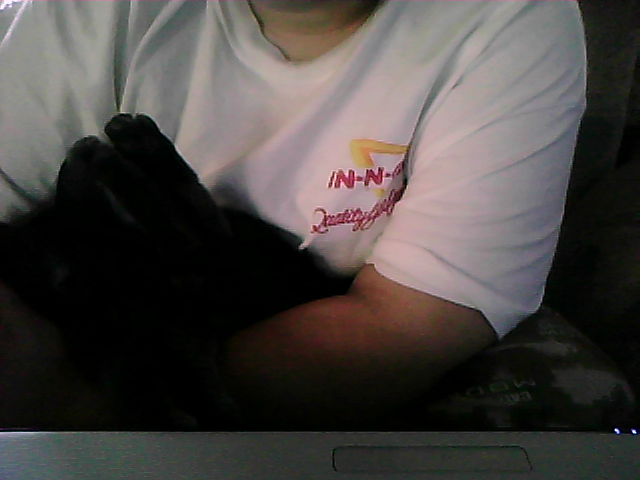
\includegraphics[width=0.5\textwidth]{original}
%	\caption{Figure 1.1. Original image}
%\end{figure}
%\begin{figure}[h]
%	\includegraphics[width=0.5\textwidth]{encoded}
%	\caption{Figure 1.2. Image encoded with a xxx byte message}
%\end{figure}
The VSL determined that there is a message about a xxx byte message in the original image. In reality, there is no message encoded into the original, but this value allows us to compare the two images. VSL determined that the modified image has a xxx byte message encoded into it. ADD VALUES AND FIX ANALYSIS Not only can steganalysis detected changes, but they are visually apparent as well. Figure 1.3 shows both an encoded image and its original.

\begin{figure}[h]
	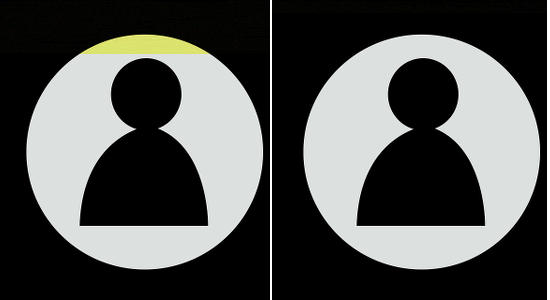
\includegraphics[width=0.5\textwidth]{comparison}
	\caption{Figure 1.3. Left: encoded, Right: original}
\end{figure}
The discoloration at the top of the encoded image is from the LSB encoding and this shows an obvious visual discoloration that an adversary can easily detect.

\subsubsection{Mitigating Risks of Steganography}
%Not enough data
These risks are mitigated by the fact that there is no universal standard for steganography methods. A user can easily replace the steganography module that we offer with a module of their own. That way, even if someone knows an image is not the original, that person will still not know who encoded it, or what kind of module was using for the encoding. Also, an encryption module can easily be added to our application and used to encrypt messages before they are encoded into an image. So even if someone knows what kind of steganography module is being used to encode messages into images, that person will also have the added challenge of decrypting the information. Although, there is no research to indicate that encryption helps in fooling steganalysis tools. Finally, since the original images exist on the internet, it will limit the plausible deniability of the user. It can be called into question as to why a certain user is uploading images that do not belong to that user to an online image database. 

%IMPLEMENTATION SECTION
\subsection{Encoding a File System}

The covert file system uses a drop in steganography module that takes in a bytearray object and returns a URL to an image. We used "least significant bit" steganography for this application because of its simplicity and reliability.

\subsubsection{Steganography Implementation}

Least significant bit (LSB) steganography is a Substitution type of steganography~\cite{Nosrati2011} that replaces the least significant bits in the image's pixels. Our steganography module is not true LSB steganography because we replace multiple bits in each pixel allowing us to encode one byte of data into every pixel. We designed our steganography technique this way to decrease the amount of images required to encode large file systems at the cost of only minimal discoloring. 

First, we break every byte of the message into three segments. Two segments of the byte will contain three bits, and the last segment will contain two bits. Next, we replace the three least significant bits of the red component with the first three bit segment. The green component follows, with the replacement of its least significant bits with the second three bit segment. Lastly, we replace the two least significant bits of the blue component with the remaining two bit segment of data. 

There are obvious drawbacks to our implementation of LSB steganography, primarily that the image may appear distorted as seen in Figure X and CovertFS images are X percent easier to detect using standard statistical analysis techniques compared to true LSB steganography as seen in figure X. However, this implementation enables us to store more bytes than other implementations of LSB steganography which decreases the latency in uploading and downloading images in large file systems [? Need evidence].
 
\subsubsection{File System to Images}

%David, I will need you to describe how the FUSE file system is prepared for encoding. Additionally, I will need information on how the files are uploaded as they are added to the file system (and future parallel upload/download). 
The first step in encoding a file system is retrieving an image. We use "The Cat API" which retrieves a random cat picture from Tumblr or a various number of other sources~\cite{CatAPIDoc}. Once we retrieve the image, we determine the number of bytes we can encode in the image by multiplying the height and width of the image, in pixels. Since we encode one byte per pixel, the result of height times width results in the total number of bytes, \textit{n}, of data we can encode in the image. For example, a 640x480 pixel image can hold 307,200 bytes of data. Next, we take the data we are going to encode and append a special end of file byte encoding. Then, we break the data into two sets, one containing the last \textit{n} bytes and the other the remaining bytes. 

Next, we encode the data in the first set into the image and upload the image. We retrieve the URL of the uploaded image and append a URL identifier byte encoding along with the URL itself to the remaining data. Then, we repeat the encoding steps by appending the end of file byte encoding, splitting the data, and uploading until there is no data left to encode. At this point, we have encoded all the data and have a "linked list" of encoded images containing the data. Finally, we can return the URL to the head image of data. 


%\section{Ethics}

%Is it ethical? Weighing the good vs the bad uses this system provides. What are the ethics of this system when we are storing our system on a social media or file sharing site (like sendspace)? 

\section{Future Implementation Plans}

One of the things we would like to implement into this project is developing the covertfs into the TAILS operating system and having it run as a bootable program through the a flash drive. The reason for this is because the TAILS operating system in and of itself offers various security measures to ensure a stable and fucntioning system. We would like to develop a working prototype where our covertfs is integrated in the TAILS operating system to further allow confidentality and plausible deniability to the users. 

The original concept paper\cite{Baliga2007}

\subsection{Encryption and Advanced Steganography Techniques}

Another future implementation worth looking into is the use of a more advanced steganographic technique. The purpose of this is to ensure the confidentiality and plausible deniability of the users by:
\begin{enumerate}
\item Ensuring that pictures being used to hide the information do not give tell-tale signs of modification
\item To increase the difficulty of steganalysis tools discovering the encrypted pictures within the sea of publicly shared images within the file sharing site or social media site that the system it using to store the file system.
\end{enumerate}

\section{Conclusion}

\section{Acknowledgments}

The original Web-Based Covert File System Paper~\cite{Baliga2007}.
\bibliographystyle{plain}
\bibliography{covertfsrefs}

\end{document}